\documentclass[11pt,a4paper]{article}


%% packages
\usepackage[utf8]{inputenc}
\usepackage[english]{babel}
\usepackage{amsfonts}
\usepackage{amsmath}
\usepackage{amssymb}
\usepackage{amsbsy}
\usepackage{authblk}
\usepackage{relsize}
\usepackage{graphicx}
\usepackage{float}
\usepackage{xcolor}
\usepackage{bbm}
\usepackage{gensymb}
\usepackage{subfigure}
\usepackage{multirow}
\usepackage{enumitem}
\usepackage{caption}
\usepackage{adjustbox}
\usepackage{comment}
\usepackage{algorithm}
\usepackage[noend]{algpseudocode}
\usepackage{url}
\usepackage{listings} % python code inserting

\definecolor{codegreen}{rgb}{0,0.6,0}
\definecolor{codegray}{rgb}{0.5,0.5,0.5}
\definecolor{codepurple}{rgb}{0.58,0,0.82}
\definecolor{backcolour}{rgb}{0.95,0.95,0.92}

\lstdefinestyle{mystyle}{
	backgroundcolor=\color{backcolour},   
	commentstyle=\color{codegreen},
	keywordstyle=\color{magenta},
	numberstyle=\tiny\color{codegray},
	stringstyle=\color{codepurple},
	basicstyle=\ttfamily\footnotesize,
	breakatwhitespace=false,         
	breaklines=true,                 
	captionpos=t,                    
	keepspaces=true,                 
	%numbers=left,                    
	numbersep=5pt,                  
	showspaces=false,                
	showstringspaces=false,
	showtabs=false,                  
	tabsize=2
}

\lstset{style=mystyle}

\renewcommand\algorithmicdo{}
\renewcommand\algorithmicthen{}
\newcommand{\xx}{\boldsymbol}
\newcommand{\yy}{\displaystyle}
\newcommand{\zz}{\widetilde}
\newcommand{\ww}{\widehat}
\makeatletter
\newcommand{\xleftrightarrow}[2][]{%
	\ext@arrow3399{\longleftrightarrowfill@}{#1}{#2}}
\newcommand{\longleftrightarrowfill@}{%
	\arrowfill@\leftarrow\relbar\rightarrow}
\makeatother

\textwidth=380pt

\font\msbmten=msbm10 scaled 1100
\def\Bbt#1{\msbmten#1}
\newcommand{\C}{\hbox{\Bbt C}}
\newcommand{\N}{\hbox{\Bbt N}}
\newcommand{\PP}{\hbox{\Bbt P}}
\newcommand{\Q}{\hbox{\Bbt Q}}
\newcommand{\R}{\hbox{\Bbt R}}
\newcommand{\Z}{\hbox{\Bbt Z}}
\newcommand{\Pol}{\hbox{\Bbt P}} 

\newcommand{\calP}{{\mathcal P}}
\newcommand{\calQ}{{\mathcal Q}} 
\newcommand{\calT}{{\mathcal T}} 
\newcommand{\calE}{{\mathcal E}} 
\newcommand{\calN}{{\mathcal N}} 

\newtheorem{prop}{Proposition}[section]
\newtheorem{rem}{Remark}[section]
\newtheorem{lem}{Lemma}[section]
\newtheorem{thm}{Theorem}[section]
\newtheorem{defn}{Definition}[section]
\newtheorem{assum}{Assumption}[section]
\newenvironment{pf}{\noindent{\bf Proof. \/}\begin{small}\noindent%
}{\hfill\EndProofMarker\end{small}}
\newcommand{\EndProofMarker}{$\Box$}

\begin{document}
\setcounter{page}{1}

\title{Modeling the cardiac action potentials in Python} 

\author[a]{Roberto Piersanti}

\affil[a]{\footnotesize Modellistica e Calcolo Scientifico (MOX), \par Dipartimento di Matematica, Politecnico di Milano, Milan, Italy}

\maketitle 

%\date{}

%\vspace*{0.5cm}

%\begin{abstract}

%\end{abstract}

\section{Introduction}\label{sec:intro}
The heart contraction is triggered by an electrical potential that propagates along all the myocardium, the cardiac muscle. The heart itself is able to produce the electrical impulse that determines this contraction. This
is possible owing to the excitability of the heart cells, the cardiomyocytes,
which, when suitably stimulated, are able to produce a variation in membrane voltage \cite{quarteroni2019}.

Differently from skeletal muscle cells, the cardiomyocyte are able to autonomously activate, independently of a nervous stimulus. The electrical activity of the heart originates at the sinoatrial node (SAN), a group of cardiac pacemaker cells located in the right atrium, see Figure~\ref{fig:heart}(a). In normal conditions, SAN cells generate an electric signal that propagates throughout the right atrium to the left atrium. The activation front reaches the atrioventricular node (AV) located at the base of the atria. The AV conducts the signal activating the specialized fibers of the Purkinje network that spread as a tree-like on the endocardial surface of the ventricles. These Purkinje terminations transmit the electric signal to the ventricular walls and cardiac excitation then propagates throughout the ventricles, see Figure~\ref{fig:heart}(a) \cite{franzone2014mathematical}. 
\begin{figure}
	\centering
	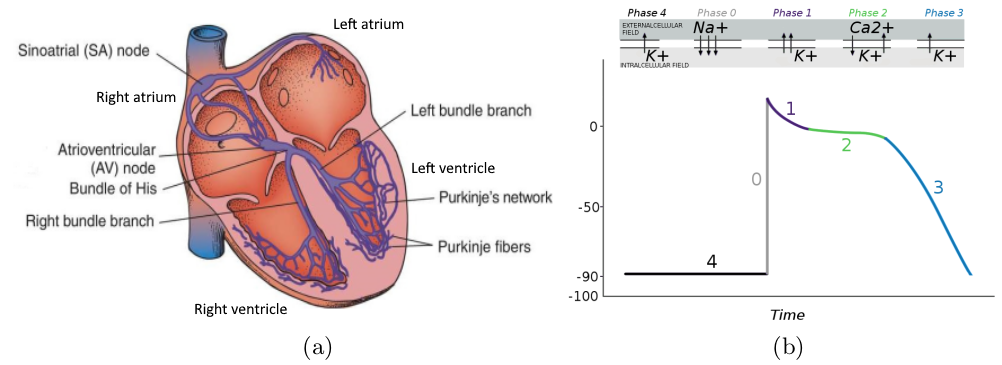
\includegraphics[width=1\textwidth]{./Images/heart_activation.png}
	\caption{The cardiac conduction system (a) and (b) the characteristic action potential of cardiomyocytes (picture taken from \cite{quarteroni2019}).}
	\label{fig:heart}
\end{figure}

\subsection{Cardiac action potentials}\label{subsec:ap}

The contraction of cardiac cells is initiated by an electrical activation due to an action potential (AP), a depolarizing transitory membrane current
that raises the transmembrane potential of an excitable cell from its resting value ranging between -90 and -80 mV to slightly positive values, followed by a repolarizing current that returns the transmembrane potential to its resting value~\cite{franzone2014mathematical}. 

At rest, the membrane potential is negative (around -90 mV), whereas when stimulated it reaches a positive value (around -20 mV) in a very short period (about 2 ms). After this depolarization, a plateau around 0 mV is observed corresponding to the refractory period, see Figure~\ref{fig:heart}(b).
Then, the repolarization phase starts, which brings the potential back to
the rest value allowing for a new excitation, see Figure~\ref{fig:heart}(b) \cite{quarteroni2019}. 

The AP is generated by several ion channels that open and close, and by
the resulting currents passing through the membrane. The most important
channels are those of calcium, sodium and potassium. In particular, a fast
inward sodium current is the main driver of rapid depolarization, a slow
inward flux of extra-cellular calcium ions is the main agent behind the characteristic plateau appearing after the depolarization, whereas the outward
potassium currents are responsible for the repolarization. The main phases of a typical cardiac AP are displayed in Figure~\ref{fig:heart}(a) \cite{quarteroni2019,franzone2014mathematical}.


\section{Cardiac mathematical cell models}\label{sec:math}
At the mathematical level, the AP is described by means of an ionic model, a system of ordinary differential equations (ODE) which models the ionic currents in the cells.

There are three families of ionic models, featuring different levels of complexity and accuracy. The first family, the so-called reduced ionic models, only provide a description of the AP and disregard sub-cellular processes. One of the most celebrated reduced model for cardiac cells is the Aliev-Panfilov (A-P) ionic model \cite{aliev1996simple}. The second family of cardiac cell models is that of the so-called first-generation models. Unlike reduced models, they allow explicit description of the kinetics of different ionic currents. Among them, the Courtemanche-Ramirez-Nattel (CRN) is the most widely used mathematical model for modeling the human atrial AP \cite{courtemanche1998ionic}. Finally, the third family of second-generation cardiac cell models, unlike first-generation models, provides a detailed description of many processes (see \cite{quarteroni2019,franzone2014mathematical} for further details). 
 
\subsection{Aliev-Panfilov ionic model}\label{subsec:aliev}
The A-P is a reduced ionic model that simulates the restitution property of cardiac tissue \cite{aliev1996simple}. It consists of two equations:
\begin{equation*}
\begin{cases}
\tfrac{\partial u}{\partial t} &= -ku(u-a)(u-1)-uv \\
\tfrac{\partial v}{\partial t} &= \epsilon(u,v)\left[ -v -ku(u-a-1)\right]
\end{cases},
\end{equation*}
where $\epsilon(u,v)=\epsilon_0+\tfrac{\mu_1 v}{u+\mu_2}$, with $k=8$, $a=0.15$, $\epsilon_0=0.002$, $\mu_1=0.2$ and $\mu_2=0.3$. The model involves dimensionless variables $u$, $v$ and $t$. The actual AP $E$, in mV, and the time $T$, in ms, can be obtained with the formulae:
$$E[mV]=100u-80, \qquad T[ms]=12.9t .$$
The model in compact form reads
\begin{equation}
\label{AP_compact}
\dfrac{\partial \mathbf{w}}{\partial t} = F(u,v),
\end{equation}
where $\mathbf{w}=[u,v]$ and $$F(u,v)=\left[-ku(u-a)(u-1)-uv,\epsilon(u,v)\left[ -v -ku(u-a-1)\right]\right].$$

\subsection{Courtemanche-Ramirez-Nattel ionic model}\label{subsec:crn}
The CRN is the most widely used mathematical model for modeling the human atrial AP \cite{courtemanche1998ionic}. The CRN was developed using specific formulations of twenty one currents based on data recorded from human atrial myocytes experiments (along with representations of pump, exchange, and background currents).

The CRN consists of twenty one ODE:
\begin{equation}
\label{crn}
\begin{cases}
\tfrac{\partial V}{\partial t} &= \dfrac{-(I_{ion}+I_{st})}{C_m} \\
\tfrac{\partial \mathbf{c}}{\partial t} &= \mathbf{F^{(c)}} \\
\tfrac{\partial \mathbf{y}}{\partial t} &= \mathbf{F^{(y)}}
\end{cases},
\end{equation}
where $V$ is the menbrane AP, the vector $\mathbf{c}=[Na, K, Ca^{2+}, Ca^{2+}_{rel}, Ca^{2+}_{up}]$ includes the ionic coentrations variable, $\mathbf{y}=[h, m, j, oa, oi, ua, ui, xr, xs, d, f, fca, u, v, w]$ is the gating varibles vector, $\mathbf{F^{(c)}}=[F_{Na}, F_{K}, F_{Ca^{2+}}, F_{Ca^{2+}_{rel}}, F_{Ca^{2+}_{up}}]$ and $\mathbf{F^{(y)}}$ (with $F_i^{(y)}=\tfrac{y_i^{\infty}-y_i}{\tau_i}$ for $i=h, m, j, oa, oi, ua, ui, xr, xs, d, f, fca, u, v, w$) are the right-hand-side (RHS) vectors of the ionic concentrations and gating varibles ODE, respectively. For the specific definition of RHS vector terms we refer to \cite{courtemanche1998ionic}. Moreover, $I_{st}$ is the applied current stimulus defined as:
$$I_{st} = -80 (\bmod(t,T_{HB}) > t^{st}_{in}) (\bmod(t,T_{HB}) < t^{st}_{end}),$$
where $T_{HB}$ is the period of one heartbeat and $t^{st}_{in}$, $t^{st}_{end}$ is the initial and final applied stimulus time, respectively. Finally, the ionic current $I_{ion}$ is defined as: 
$$I_{ion}=I_{Na}+I_{K1}+I_{to}+I_{Kur}+I_{Kr}+I_{Ks}+I_{Ca,L}+I_{p,Ca}+I_{NaK}+I_{NaCa}+I_{b,Na}+I_{b,Ca},$$
where for the specific definition of each term in $I_{ion}$ we refer to \cite{courtemanche1998ionic}. 

\noindent
The model \eqref{crn} in compact form reads
\begin{equation}
\label{crn_compact}
\dfrac{\partial \mathbf{Y}}{\partial t} = \mathbf{F},
\end{equation}
where $\mathbf{Y}=[V,\mathbf{c},\mathbf{y}]$ and $\mathbf{F}=\left[ \tfrac{-(I_{ion}+I_{st})}{C_m}, \mathbf{F^{(c)}}, \mathbf{F^{(y)}} \right]$.

\section{Python implementation}\label{sec:python}
In the following section we detail the Python implementation for the A-P and CRN ionic models introduced in Section \ref{sec:math}. 

\subsection{Aliev-Panfilov code}\label{subsec:python_ap}
To numerically solve the AP model in Python we use the \verb|scipy.integrate| package using the function \verb|odeint|.

\lstset{language=Python}
\lstset{frame=lines}
%\lstset{caption={Insert code directly in your document}}
%\lstset{label={lst:code_direct}}
\lstset{basicstyle=\footnotesize}
\begin{lstlisting}
y = odeint(model, y0, t)
\end{lstlisting}
The \verb|odeint| requires three inputs: 
\begin{itemize}
	\item \verb|model|: function name that returns derivative values at requested y and t values as dydt = model(y,t);
	\item \verb|y0|: initial conditions of the differential states;
	\item \verb|t|: time points at which the solution should be reported.
\end{itemize}
An example of using \verb|odeint| is the following differential equation: 
\begin{equation}
\label{ex_odeint}
\dfrac{d y(t)}{d t} = -ky(t),
\end{equation}
with parameter $k=0.3$, the initial condition $y0=5$. The Python code (1) first imports the needed \verb|Numpy|, \verb|Scipy|, and \verb|Matplotlib| packages.  The model, initial conditions, and time points are defined as inputs to \verb|odeint| to numerically calculate $y(t)$.
\begin{figure}
	\centering
	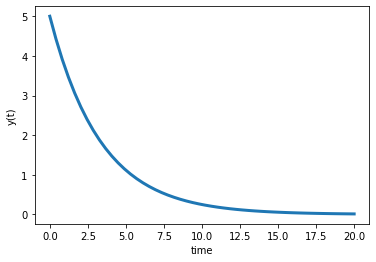
\includegraphics[width=0.75\textwidth]{./Images/odeint_ex.png}
	\caption{Result of code (1) for solving the equation \eqref{ex_odeint} with odeint.}
	\label{fig:ex_odeint}
\end{figure}  

\lstset{language=Python}
\lstset{frame=lines}
\lstset{caption={example of using odeint for the example equation \eqref{ex_odeint}}}
\lstset{basicstyle=\footnotesize}
\begin{lstlisting}
import numpy as np
from scipy.integrate import odeint

# function that returns dy/dt
def model(y,t):
	k = 0.3
	dydt = -k * y
	return dydt

# initial condition
y0 = 5

# time points
t = np.linspace(0,20)

# solve ODE
y = odeint(model,y0,t)
\end{lstlisting}
Figure \ref{fig:ex_odeint}, produced by means of code (2), shows the result of code (1).

\lstset{language=Python}
\lstset{frame=lines}
\lstset{caption={Plot the result of code (1)}}
%\lstset{label={lst:code_direct}}
\lstset{basicstyle=\footnotesize}
\begin{lstlisting}
import matplotlib.pyplot as plt

plt.plot(t,y,linewidth=3)
plt.xlabel('time')
plt.ylabel('y(t)')
plt.show()
\end{lstlisting}
\newpage

The Python code (3) implements the A-P ionic model using the \verb|odeint| package. The model, initial conditions, and time points are defined as inputs to \verb|odeint| to numerically calculate the solution of equation \eqref{AP_compact}.

\lstset{language=Python}
\lstset{frame=lines}
\lstset{caption={A-P ionic model Python code}}
\lstset{basicstyle=\footnotesize}
\begin{lstlisting}
import numpy as np  
from scipy.integrate import odeint 

def AP_model(k=8, a=0.15, eps_0=0.002, mu_1=0.2, mu_2=0.3):
	def eps_fun(u, v):
		return eps_0 + mu_1*v/(u+mu_2)

	def fun(y, t):
		u, v = y
		eps = eps_fun(u,v)
		dydt = [-k*u*(u-a)*(u-1)-u*v, eps*(-v-k*u*(u-a-1))]
		return dydt
	return fun

def u_to_mV(u):
	return 100 * u - 80

def t_to_ms(t):
	return 12.9 * t

def run():
	t_0 = 0
	t_end = 40
	discretization = (t_end - t_0) * 1000
	t = np.linspace(t_0, t_end, discretization)
	y0 = (0.17, 0)
	solution = odeint(AP_model(), y0, t)
\end{lstlisting}

\subsection{Courtemanche-Ramirez-Nattel code}\label{subsec:python_crn}
The Python code for solving the CRN ionic model begins with the model constants definition after importing the needed \verb|Numpy| package:
\lstset{language=Python}
\lstset{frame=lines}
\lstset{caption={CRN constants definition}}
\lstset{basicstyle=\footnotesize}
\begin{lstlisting}
import numpy as np  
import matplotlib.pyplot as plot
log = np.log;
exp = np.exp;
sqrt = np.sqrt;

# constants 
R = 8.3143;        # Gas constant 
T = 310;           # Temperature  
Fconst = 96.4867;  # Faraday constant 
Vi = 13668;        # Intracellular volume 
Vup = 1109.52;     # Sarcoplasmic Reticulum uptake volume 
Vrel = 96.48;      # Sarcoplasmic Reticulum release volume
K0 = 5.4;          # Extracellular K+ concentration 
Na0 = 140;         # Extracellular Na+ concentration
Ca0 = 1.8;         # Extracellular Ca2+ concentration 
gna = 7.8;         # Maximal I_Na conductance 
gk1 = 0.09;        # Maximal I_K1 conductance 
gto = 0.1652;      # Maximal I_to conductance 
gkr = 0.0294;      # Maximal I_Kr conductance 
gks = 0.129;       # Maximal I_Ks conductance 
gcal = 0.1238;     # Maximal I_Cal conductance 
gbca = 0.00113;    # Maximal I_bCa conductance 
gbna = 0.000674;   # Maximal I_bNa conductance 
Inakmax = 0.60;    # Maximal I_NaK 
Inacamax = 1600;   # Maximal I_NaCa 
Ipcamax = 0.275;   # Maximal I_pCa 
Iupmax = 0.005;    # Maximal I_up 
KQ10 = 3;          # Temperature scaling for I_Kur and I_to                    
gamma = 0.35;      # Voltage dependence param for I_NaCa 
Kmnai = 10;        # [Na+]i Half saturation constant for I_NaK
Kmko = 1.5;        # [K+]o  Half saturation constant for I_NaK 
Kmna = 87.5;       # [Na+]o Half saturation constant for I_NaCa 
Kmca = 1.38;       # [Ca2+]o Half saturation constant for I_NaCa 
ksat = 0.1;        # Saturation factor for I_NaCa
krel = 30;         # Maximal release rate for I_rel 
kup = 0.00092;     # [Ca2+]o half-saturation constant for I_up 
Caupmax = 15;      # Maximal Ca2+ conc in uptake compartement 
Cmdnmax = 0.05;    # Total calmodulin concentration in myoplasm 
Trpnmax = 0.07;    # Total troponin concentration in myplasm 
Csqnmax = 10;      # Total calsequestrin concentration in myoplasm 
Kmcmdn = 0.00238;  # [Ca2+]i half saturation constant for calmodulin 
Kmtrpn = 0.0005;   # [Ca2+]i half saturation constant for troponin 
Kmcsqn = 0.8;      # [Ca2+]rel half saturation constant for I_up 

Cm     = 1;        # Membrane capacitance
CCconv = 1e6*2e-4; # Conversion factor  
\end{lstlisting}
Then there is the defininion of the CRN initial conditions:
\lstset{language=Python}
\lstset{frame=lines}
\lstset{caption={CRN initial conditions}}
\lstset{basicstyle=\footnotesize}
\begin{lstlisting}
y0 = np.zeros(21);
y0[0] = -81.2;          # v
y0[1] = 11.2;           # Na
y0[2] = 139;            # K
y0[3] = 1.02*1e-4;      # Ca2+
y0[4] = 1.49;           # Ca2+rel
y0[5] = 1.49;           # Ca2+up
y0[6] = 0.965;          # h
y0[7] = 2.91 * 1e-03;   # m
y0[8] = 0.978;          # j
y0[9]= 3.04 * 1e-02;    # oa
y0[10]= 0.999;          # oi
y0[11]= 4.96*1e-3;      # ua
y0[12]= 0.999;          # ui
y0[13]= 3.29*1e-5;      # xr
y0[14]= 0.0187;         # xs
y0[15]= 1.37*1e-4;      # d
y0[16]= 0.999;          # f
y0[17]= 0.775;          # fca
y0[18]= 0.0;            # u
y0[19]= 1.0;            # v
y0[20]= 0.999;          # w
\end{lstlisting}
The ionic currents definition follows: 
\lstset{language=Python}
\lstset{frame=lines}
\lstset{caption={CRN ionic currents}}
\lstset{basicstyle=\footnotesize}
\begin{lstlisting}
def ENa(y):
	return R * T/Fconst * log(Na0/y[1])
def EK(y):
	return R * T/Fconst * log(K0/y[2]) 
def ECa(y):
	return R * T/(2*Fconst) * log(Ca0/y[3]) 

def INa(y):
	return gna * y[7]**3 * y[6] * y[8] * (y[0] - ENa(y)) 
def IK1(y):
	return gk1 * (y[0] - EK(y)) / (1 + exp(0.07 * (y[0] + 80))) 
def Ito(y):
	return gto * y[9]**3 * y[10] * (y[0] - EK(y))
def gkur(y):
	return 0.005 + 0.05 / (1 + exp(-(y[0]-15)/13))
def Ikur(y):
	return gkur(y) * y[11]**3 * y[12] * (y[0] - EK(y))
def IKr(y):
	return gkr * y[13] * (y[0] - EK(y)) / (1 + exp((y[0] + 15)/22.4))
def IKs(y):
	return gks * y[14]**2 * (y[0] - EK(y))
def ICaL(y):
	return gcal * y[15] * y[16] * y[17] * (y[0] - 65)
def fnak(y):
	return 1 / (1 + 0.1245 * exp(-0.1*Fconst*y[0]/R/T) + 0.0365 / 7 * (exp(Na0/67.3) - 1) * exp(-Fconst*y[0]/R/T))
def INaK(y):
	return Inakmax * fnak(y) * K0 / (1 + (Kmnai/y[1])**1.5) / (K0 + Kmko) 
def INaCanum(y):
	return Inacamax * (exp(gamma * Fconst * y[0]/R/T)*y[1]**3*Ca0 - exp((gamma-1)*Fconst*y[0]/R/T)*Na0**3*y[3])
def INaCaden(y):
	return (Kmna**3 + Na0**3)*(Kmca + Ca0)*(1 + ksat*(exp((gamma-1)*Fconst*y[0]/R/T)))
def INaCa(y):
	return INaCanum(y) / INaCaden(y)
def Ibca(y):
	return gbca * (y[0] - ECa(y))
def Ibna(y):
	return gbna * (y[0] - ENa(y))
def Ipca(y):
	return Ipcamax * y[3]/ (0.0005 + y[3])
def Irel(y):
	return krel * y[18]**2 * y[19] * y[20] * (y[4] - y[3])
def Itr(y):
	return (y[5] - y[4]) / 180
def Iup(y):
	return Iupmax / (1 + (kup/y[3]))
def Iupleak(y):
	return y[5] * Iupmax / Caupmax

def Iion(y):
	return INa(y) + IK1(y) + Ito(y) + Ikur(y) + IKr(y) + IKs(y) + ICaL(y) + Ipca(y) + INaK(y) + INaCa(y) + Ibna(y) + Ibca(y)
def Ist(t):
	return -80 * (t%THB < 21) * (t%THB > 20)
\end{lstlisting}
Then there is the RHS definition of the AP equation: 
\lstset{language=Python}
\lstset{frame=lines}
\lstset{caption={CRN RHS of the AP equation}}
\lstset{basicstyle=\footnotesize}
\begin{lstlisting}
def Vfunc(t,y):
	return -(Iion(y) + Ist(t))/Cm
\end{lstlisting}
The gating variables definition follows: 
\lstset{language=Python}
\lstset{frame=lines}
\lstset{caption={CRN gating variables}}
\lstset{basicstyle=\footnotesize}
\begin{lstlisting}
#hfunc
def alphah(y):
	return 0.135*exp( -(y[0] + 80)/6.8) * (y[0] < -40) 
def betah(y):
	return 3.56 * exp(0.079*y[0]) + 3.1*1e5 * exp(0.35 * y[0]) * (y[0] < -40) + (y[0] >= -40) * 1/0.13 / (1 + exp(-(y[0]+10.66) / 11.1))
def tauh(y):
	return 1 / (alphah(y) + betah(y))
def hinf(y):
	return alphah(y) * tauh(y)
def hfunc(y):
	return (hinf(y) - y[6]) / (tauh(y))
#mfunc
def alpham(y):
	return 0.32 * (y[0] + 47.13) / (1 - exp(-0.1*(y[0] + 47.13))) * (y[0] != -47.13) + (y[0] == -47.13) * 3.2
def betam(y):
	return 0.08 * exp(-y[0]/11)
def taum(y):
	return 1 / (alpham(y) + betam(y))
def minf(y):
	return alpham(y) * taum(y)
def mfunc(y):
	return (minf(y) - y[7]) / (taum(y))
#jfunc
def alphaj(y):
	return (-126140 * exp(0.2444*y[0]) - 3.474 * 1e-5 * exp(-0.04391*y[0])) * (y[0] + 37.78)/(1 + exp(0.311*(y[0] + 79.23))) * (y[0] < -40)
def betaj(y):
	return 0.1212 * exp(-0.01052*y[0]) / (1 + exp(-0.1378*(y[0] + 40.14))) * (y[0] < -40) + 0.3 * exp(-2.535 * 1e-7)/(1 + exp(-0.1 * (y[0] + 32))) * (y[0] >= -40)
def tauj(y):
	return 1 / (alphaj(y) + betaj(y))
def jinf (y):
	return alphaj(y) * tauj(y)
def jfunc(y):
	return (jinf(y) - y[8]) / (tauj(y))
#oafunc
def alphaoa(y):
	return 0.65 / (exp(-(y[0] + 10)/8.5) + exp(-(y[0] - 30)/59.0))
def betaoa(y):
	return 0.65 / (2.5 + exp((y[1] + 82)/17))
def tauoa(y):
	return 1 / (alphaoa(y) + betaoa(y)) / KQ10
def oainf(y):
	return 1 / (1 + exp(-(y[0] + 20.47)/17.54))
def oafunc(y):
	return (oainf(y) - y[9]) / (tauoa(y))
#oifunc
def alphaoi(y):
	return 1 / (18.53 + exp((y[0] + 113.7)/10.95))
def betaoi(y):
	return  1 / (35.56 + exp(-(y[0] + 1.26)/7.44))
def tauoi(y):
	return 1 / (alphaoi(y) + betaoi(y)) / KQ10
def oiinf(y):
	return 1 / (1 + exp((y[0] + 43.1)/5.3))
def oifunc(y):
	return (oiinf(y) - y[10]) / (tauoi(y))
#uafunc
def alphaua(y):
	return 0.65 / (exp(-(y[0] + 10)/8.5) + exp(-(y[0]-30)/59))
def betaua(y):
	return 0.65 / (2.5 + exp((y[0] + 82)/17))
def tauua(y):
	return 1 / (alphaua(y) + betaua(y)) / KQ10
def uainf(y):
	return 1 / (1 + exp(-(y[1] + 30.3)/9.6))
def uafunc(y):
	return (uainf(y) - y[11]) / (tauua(y))
#uifunc
def alphaui(y):
	return 1 / (21 + exp(-(y[0]-185)/28))
def betaui(y):
	return exp((y[0]-158)/16)
def tauui(y):
	return 1 / (alphaui(y) + betaui(y)) / KQ10
def uiinf(y):
	return 1 / (1 + exp((y[0] - 99.45)/27.48))
def uifunc(y):
	return (uiinf(y) - y[12]) / (tauui(y))
#xrfunc 
def alphaxr(y):
	return 0.0003 * (y[0] + 14.1) / (1 - exp(-(y[0] + 14.1)/5))
def betaxr(y):
	return 7.3898 * 1e-5 * (y[0] - 3.3328) / (exp((y[0] - 3.3328)/5.1237) - 1)
def tauxr(y):
	return 1 / (alphaxr(y) + betaxr(y))
def xrinf(y):
	return 1 / (1 + exp(-(y[0] + 14.1)/6.5))
def xrfunc(y):
	return (xrinf(y) - y[13]) / (tauxr(y))
#xs func
def alphaxs(y):
	return 4 * 1e-5 * (y[0] - 19.9) / (1 - exp(-(y[0]-19.9)/17))
def betaxs(y):
	return 3.5 * 1e-5 * (y[0]-19.9) / (exp((y[0]-19.9)/9) - 1)
def tauxs(y):
	return 0.5 / (alphaxs(y) + betaxs(y))
def xsinf(y):
	return 1 / sqrt(1 + exp(-(y[0] - 19.9)/12.7))
def xsfunc(y):
	return (xsinf(y) - y[14]) / (tauxs(y))
#dfunc
def taud(y):
	return (1 - exp(-(y[0]+10)/6.24)) / (0.035*(y[0] + 10)*(1 + exp(-(y[0] + 10)/6.24)))
def dinf(y):
	return 1 / (1 + exp(-(y[0] + 10)/8))
def dfunc(y):
	return (dinf(y) - y[15]) / (taud(y))
#ffunc
def tauf(y):
	return 9 / (0.0197 * exp(-0.0337 * 0.0337 * (y[0]+10)**2) + 0.02)
def finf(y):
	return 1 / (1 + exp((y[0]+28)/6.9))
def ffunc(y):
	return (finf(y) - y[16]) / (tauf(y))
#fca func
def fcainf(y):
	return 1 / (1 + y[3]/0.00035)
def fcafunc(y):
	return (fcainf(y) - y[17]) / 2
#ufunc
def Fn(y):
	return 1e-12 * Vrel * Irel(y) - 5*1e-13/Fconst*(0.5 * ICaL(y)-INaCa(y)/5)
def uinf(y):
	return 1 / (1 + exp(-(Fn(y)-3.4175 * 1e-13) / (13.67 * 1e-16)))
def ufunc(y):
	return (uinf(y) - y[18]) / 8
#vfunc
def tauv(y):
	return 1.91 + 2.09 / (1 + exp(-(Fn(y) - 3.4175 * 1e-13)/(13.67 * 1e-16)))
def vinf(y):
	return 1 - 1 / (1 + exp(-(Fn(y) - 6.835 * 1e-14)/(13.67 * 1e-16)))
def vfunc(y):
	return (vinf(y) - y[19]) / tauv(y)
#wfunc
def tauw(y):
	return 6.0 * (1 - exp(-(y[0]-7.9)/5)) / (1 + 0.3 * exp(-(y[0]-7.9)/5)) / (y[0] - 7.9)
def winf(y):
	return 1 - 1 / (1 + exp(-(y[0] - 40)/17))
def wfunc(y):
	return (winf(y) - y[20]) / tauw(y)
\end{lstlisting}
Defining the RHS of the concentration equations:
\lstset{language=Python}
\lstset{frame=lines}
\lstset{caption={RHS of the concentration equations}}
\lstset{basicstyle=\footnotesize}
\begin{lstlisting}
def Nafunc(y):
	return CCconv * (-3*INaK(y) - 3*INaCa(y) - Ibna(y) - INa(y)) / (Fconst*Vi)
def Kfunc(y):
	return CCconv * (2*INaK(y) - IK1(y) - Ito(y) - Ikur(y) - IKr(y) - IKs(y)) / (Fconst*Vi)
def B1(y):
	return CCconv * (2*INaCa(y) - Ipca(y) - ICaL(y) - Ibca(y))/(2*Fconst*Vi) + (Vup*(Iupleak(y) - Iup(y)) + Irel(y)*Vrel)/Vi
def B2(y):
	return 1 + Trpnmax*Kmtrpn/(y[3] + Kmtrpn)**2 + Cmdnmax * Kmcmdn/(y[3] + Kmcmdn)**2
def Cafunc(y):
	return B1(y)/B2(y)
def Caupfunc(y):
	return Iup(y) - Iupleak(y) - Itr(y) * Vrel / Vup
def Carelfunc(y):
	return (Itr(y) - Irel(y))/(1 + Csqnmax * Kmcsqn/(y[4] + Kmcsqn)**2)
\end{lstlisting}
Defining the RHS of of all the ODE:
\lstset{language=Python}
\lstset{frame=lines}
\lstset{caption={Vector of RHS of all the ODE}}
\lstset{basicstyle=\footnotesize}
\begin{lstlisting}
def F(t,y):
	vF = np.array((Vfunc(t,y), Nafunc(y), Kfunc(y), Cafunc(y), Carelfunc(y), Caupfunc(y), hfunc(y), mfunc(y), jfunc(y), oafunc(y), oifunc(y), uafunc(y), uifunc(y), xrfunc(y), xsfunc(y), dfunc(y), ffunc(y), fcafunc(y), ufunc(y), vfunc(y), wfunc(y)));
	return vF
\end{lstlisting}
Finally, the CRN model \eqref{crn_compact} is numerically solved by means of the forward Euler method. Introducing the discrete times $t^n=n dt$  (where $dt=\frac{t_{end}-t_{0}}{n}$ with $t_0$, $t_{end}$ the initial and final times, respectively and $n \in \mathbb {N}_0^+$) and denoting $\mathbf{A}^{n}$ the time discretization of the generic vector variable $\mathbf{A}$, one step of the Euler method from $t_n=t_0 + ndt$ to $t_{n+1}=t_0 + (n+1)dt$ is: 
\begin{equation}
\label{crn_time}
\mathbf{Y}^{n+1}=\mathbf{Y}^{n}+dt\mathbf{F}^n.
\end{equation}
The time discretization \eqref{crn_time} is perfomed by means of code (11).

\lstset{language=Python}
\lstset{frame=lines}
\lstset{caption={CRN ionic model time integration}}
\lstset{basicstyle=\footnotesize}
\begin{lstlisting}
THB = 800;         # heartbeat length      [ms]
nHB = 1;           # number of heartbeats  [-]

t_in = 0;                           # initial time
dt = 0.01;                          # time step
t_end = nHB * THB;                  # final time
tt = np.arange(t_in, t_end+dt, dt); # time vector

dim = y0.size;  
Y = np.zeros((dim,tt.size)); # Inizialize solution
Y[:,0] = y0;                 # Vector of initial conditions

index = 1;
t = t_in;
for i in tt[1:]:
	y0 = y0 + dt * F(i,y0);
	Y[:,index] = y0;
	t = t + dt;
	index = index + 1;
\end{lstlisting}

\section{Numerical results}\label{sec:results}

In this section we show the results obtained with the A-P and CRN codes fully detailed in Section \ref{sec:python}.

\subsection{Aliev-Panfilov}\label{sec:results_ap}

Figure \ref{fig:ap}, obtained by means of the plotter code (12), display the time trace of the AP (both in dimensional and adimensional forms), the gating variable and the phase diagram for the A-P ionic model.  

\begin{figure}[t]
	\centering
	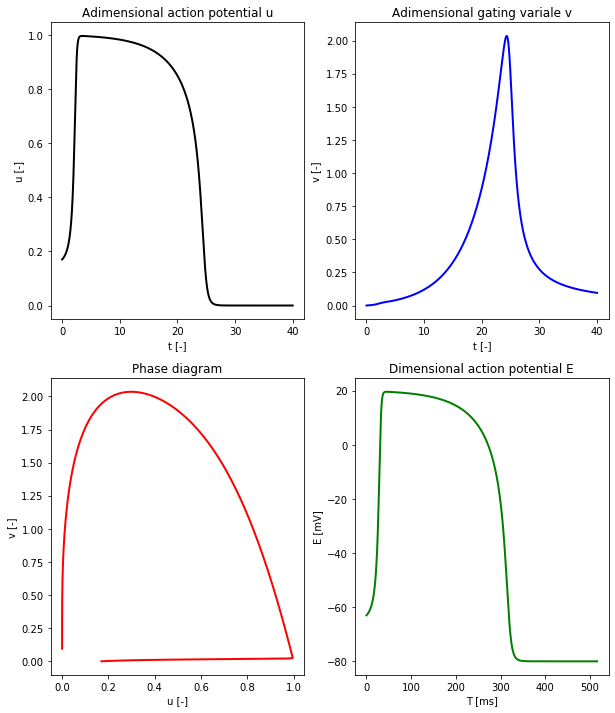
\includegraphics[width=0.85\textwidth]{./Images/A-P.png}
	\caption{Result of the A-P code.}
	\label{fig:ap}
\end{figure} 

\lstset{language=Python}
\lstset{frame=lines}
\lstset{caption={A-P plotter}}
\lstset{basicstyle=\footnotesize}
\begin{lstlisting}
import matplotlib.pyplot as plot  

def pictures(t, solution):
fig = plot.figure(1, figsize=(10, 12))

ax1 = fig.add_subplot(221)
ax1.plot(t, solution[:, 0],'k',linewidth=2)
ax1.set_title('Adimensional action potential u')
ax1.set_xlabel('t [-]')
ax1.set_ylabel('u [-]')

ax2 = fig.add_subplot(222)
ax2.plot(t, solution[:, 1],'b',linewidth=2)
ax2.set_title('Adimensional gating variale v')
ax2.set_xlabel('t [-]')
ax2.set_ylabel('v [-]')

ax3 = fig.add_subplot(223)
ax3.plot(solution[:, 0], solution[:, 1],'r',linewidth=2)
ax3.set_title('Phase diagram')
ax3.set_xlabel('u [-]')
ax3.set_ylabel('v [-]')

E = u_to_mV(solution[:, 0])
T = t_to_ms(t)

ax4 = fig.add_subplot(224)
ax4.set_title('Dimensional action potential E')
ax4.plot(T, E,'g',linewidth=2)
ax4.set_xlabel('T [ms]')
ax4.set_ylabel('E [mV]')

plot.show()
\end{lstlisting}
\begin{figure}[ht!]
	\centering
	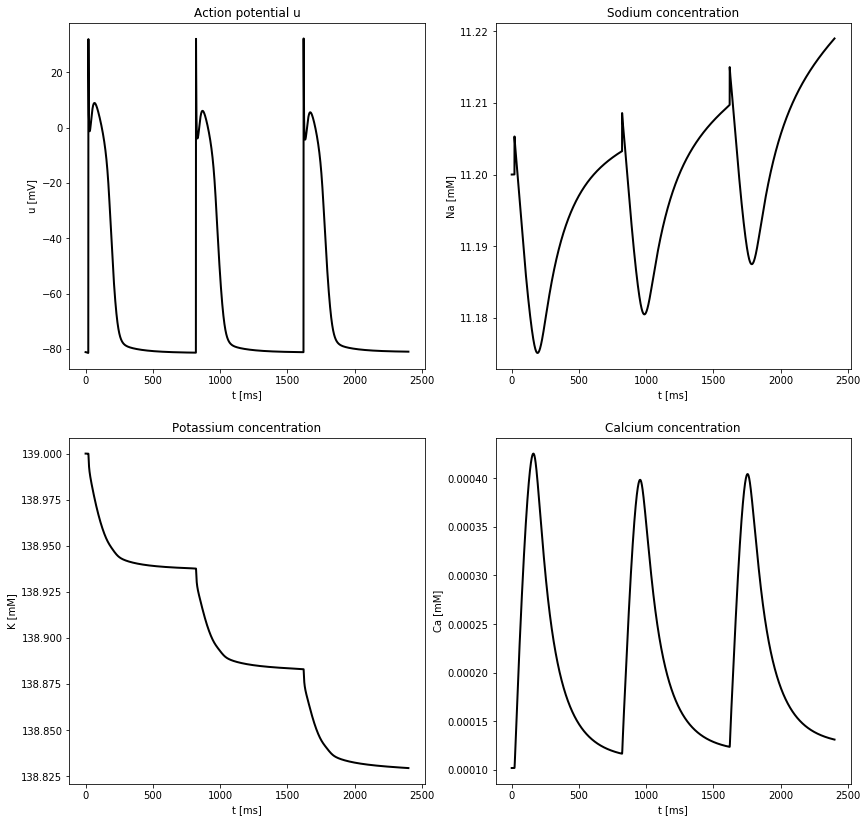
\includegraphics[width=1\textwidth]{./Images/CRN.png}
	\caption{Result of the CRN code.}
	\label{fig:crn}
\end{figure} 
\subsection{Courtemanche-Ramirez-Nattel}\label{sec:results_ap}
Figure \ref{fig:crn}, obtained by means of the plotter code (13), display the time trace of the AP and three concentrations (Sodium, Potassium and Calcium) of the CRN ionic model.  

\newpage
\lstset{language=Python}
\lstset{frame=lines}
\lstset{caption={CRN plotter}}
\lstset{basicstyle=\footnotesize}
\begin{lstlisting}
import matplotlib.pyplot as plot  

def pictures(time, solution):
fig = plot.figure(1, figsize=(14, 14))

ax1 = fig.add_subplot(221)
ax1.plot(time, solution[0,:],'k',linewidth=2)
ax1.set_title('Action potential u')
ax1.set_xlabel('t [ms]')
ax1.set_ylabel('u [mV]')

ax2 = fig.add_subplot(222)
ax2.plot(time, solution[1,:],'k',linewidth=2)
ax2.set_title('Sodium concentration')
ax2.set_xlabel('t [ms]')
ax2.set_ylabel('Na [mM]')

ax3 = fig.add_subplot(223)
ax3.plot(time, solution[2,:],'k',linewidth=2)
ax3.set_title('Potassium concentration')
ax3.set_xlabel('t [ms]')
ax3.set_ylabel('K [mM]')

ax4 = fig.add_subplot(224)
ax4.set_title('Calcium concentration')
ax4.plot(time, solution[3,:],'k',linewidth=2)
ax4.set_xlabel('t [ms]')
ax4.set_ylabel('Ca [mM]')

plot.show()
\end{lstlisting}

%\clearpage

\bibliographystyle{unsrt} % cite order  
\bibliography{latexbib}

\end{document}